\documentclass{report}

\usepackage{amsmath}
\usepackage{geometry}
\usepackage{amsfonts}
\usepackage[english]{babel}
\usepackage{amssymb}
\usepackage{graphicx}
\usepackage{float}
\usepackage{hyperref}
\usepackage{multirow}
\usepackage{pdflscape}
\usepackage{caption}
\usepackage{pdflscape}
\usepackage{outlines}
\usepackage{subcaption}
\usepackage{enumerate}
\usepackage[latin1]{inputenc}

\usepackage{tabularx, booktabs}
\usepackage{longtable}

\usepackage{standalone}

\usepackage[autostyle, english = american]{csquotes}
\MakeOuterQuote{"}

\usepackage{comment}

\newcommand{\tabnotes}[2]{\bottomrule \multicolumn{#1}{@{}p{0.95\linewidth}@{}}{\footnotesize #2 }\end{tabular}\end{table}}

\title{Defense Spending Spillovers}
\author{Isaac Liu}
\date{\today}

\setlength{\parindent}{0pt}
\setlength{\parskip}{0.5em}

\hypersetup{
    colorlinks=true,
    linkcolor=blue,
    filecolor=magenta,      
    urlcolor=cyan,
}

\begin{document}

	\maketitle

	\newpage \clearpage

    \section*{Idea}

	We examine spillovers/relationships between military spending among countries using the PCA/Factor methods and potentially the LASSO. Using PCA we can summarize the relationships in spending among countries or over time and possibly attach interpretations or labels to key factors. Using the LASSO, regressing an individual country's spending on that of other countries, we can see which countries impact or are impacted by others.

	A hypothesis is that spending in neighboring countries increases local spending. Yet another hypothesis is that ideological differences/alignment are somehow related. We can also check to see if the US, Russia, or other countries have disproportionate influence. It's also possible that key factors change from period to period- post Cold War to Post 9/11, for example.

    \section*{Literature}

	In the literature, the main approach to examining military spending appears to be spatial autoregression: \url{https://www.sciencedirect.com/science/article/pii/S0176268017301581}. I haven't seen anything using machine learning methods, even though I flipped through 10 Google Scholar pages. Though, here's a triple LASSO involving military spending but the question is different (it's looking at the fiscal multiplier): \url{https://papers.ssrn.com/sol3/papers.cfm?abstract_id=3819192}.

	Our approach will allow us to look at potentially both spatial and ideological factors. Machine learning methods will also allow us to take a unique approach of imposing sparsity and dimension reduction (a country's spending is only affected by a few others, or is explained by only a couple key factors).

	This question presents some unique challenges as to dealing with pretty limited panel data: a small sample size with a lot of missing values, which provide space for unique methods.

	\newpage \clearpage

    \section*{Military Expenditure Data}

    Our data on military expenditure as a percentage of GDP comes from SIPRI, the Stockholm International
	Peace Research Institute. There are several other series available, such as spending in absolute terms or as a share of the government budget. We have also download the Varieties of Democracy dataset, which contains information on hundreds of political variables and indicators for ethnic conflict and other measures, which could lead to heterogenous impacts on spending.

	\begin{figure}[h!]
		\centering
		\caption{Military Expenditure as Percentage of GDP Time Series for Countries}
		\label{Milex_GDP_Time_Series}	
		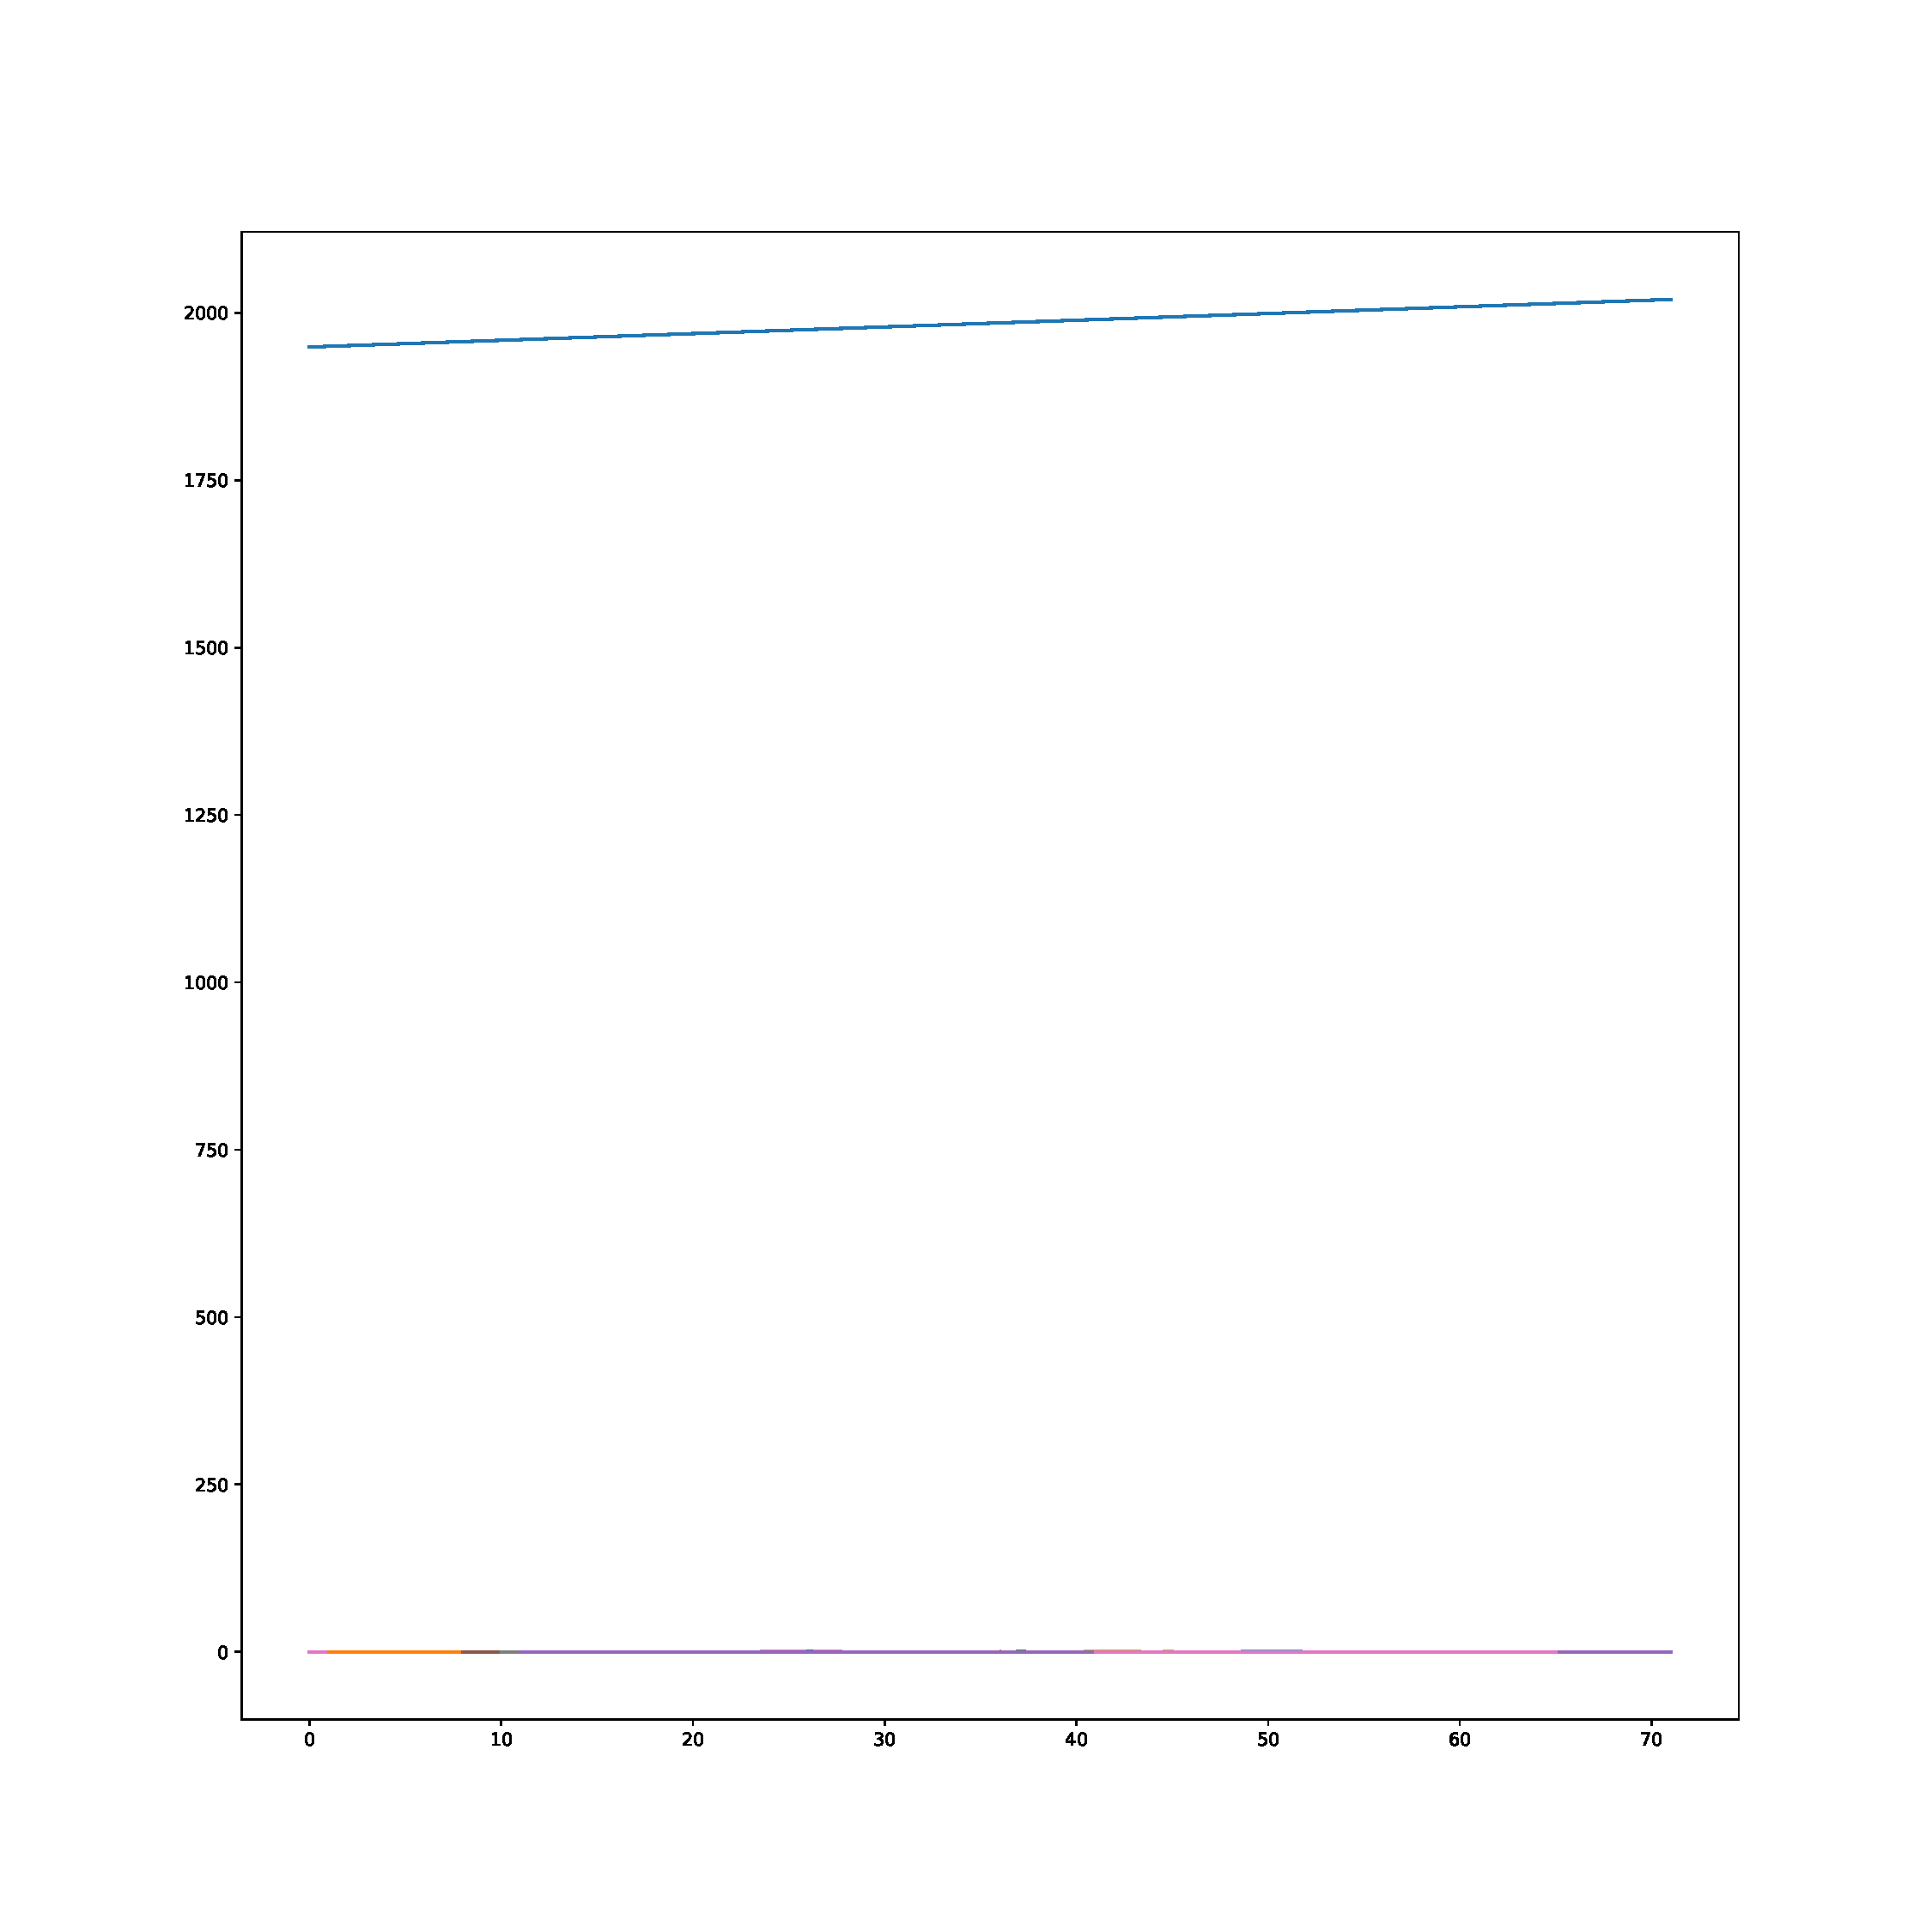
\includegraphics[width=\linewidth,keepaspectratio=true]{../Output/Figures/Milex_GDP_Time_Series.pdf}
	\end{figure}

	\begin{figure}[h!]
		\centering
		\caption{Correlations Between Country Military Spending}
		\label{Milex_Correlations}	
		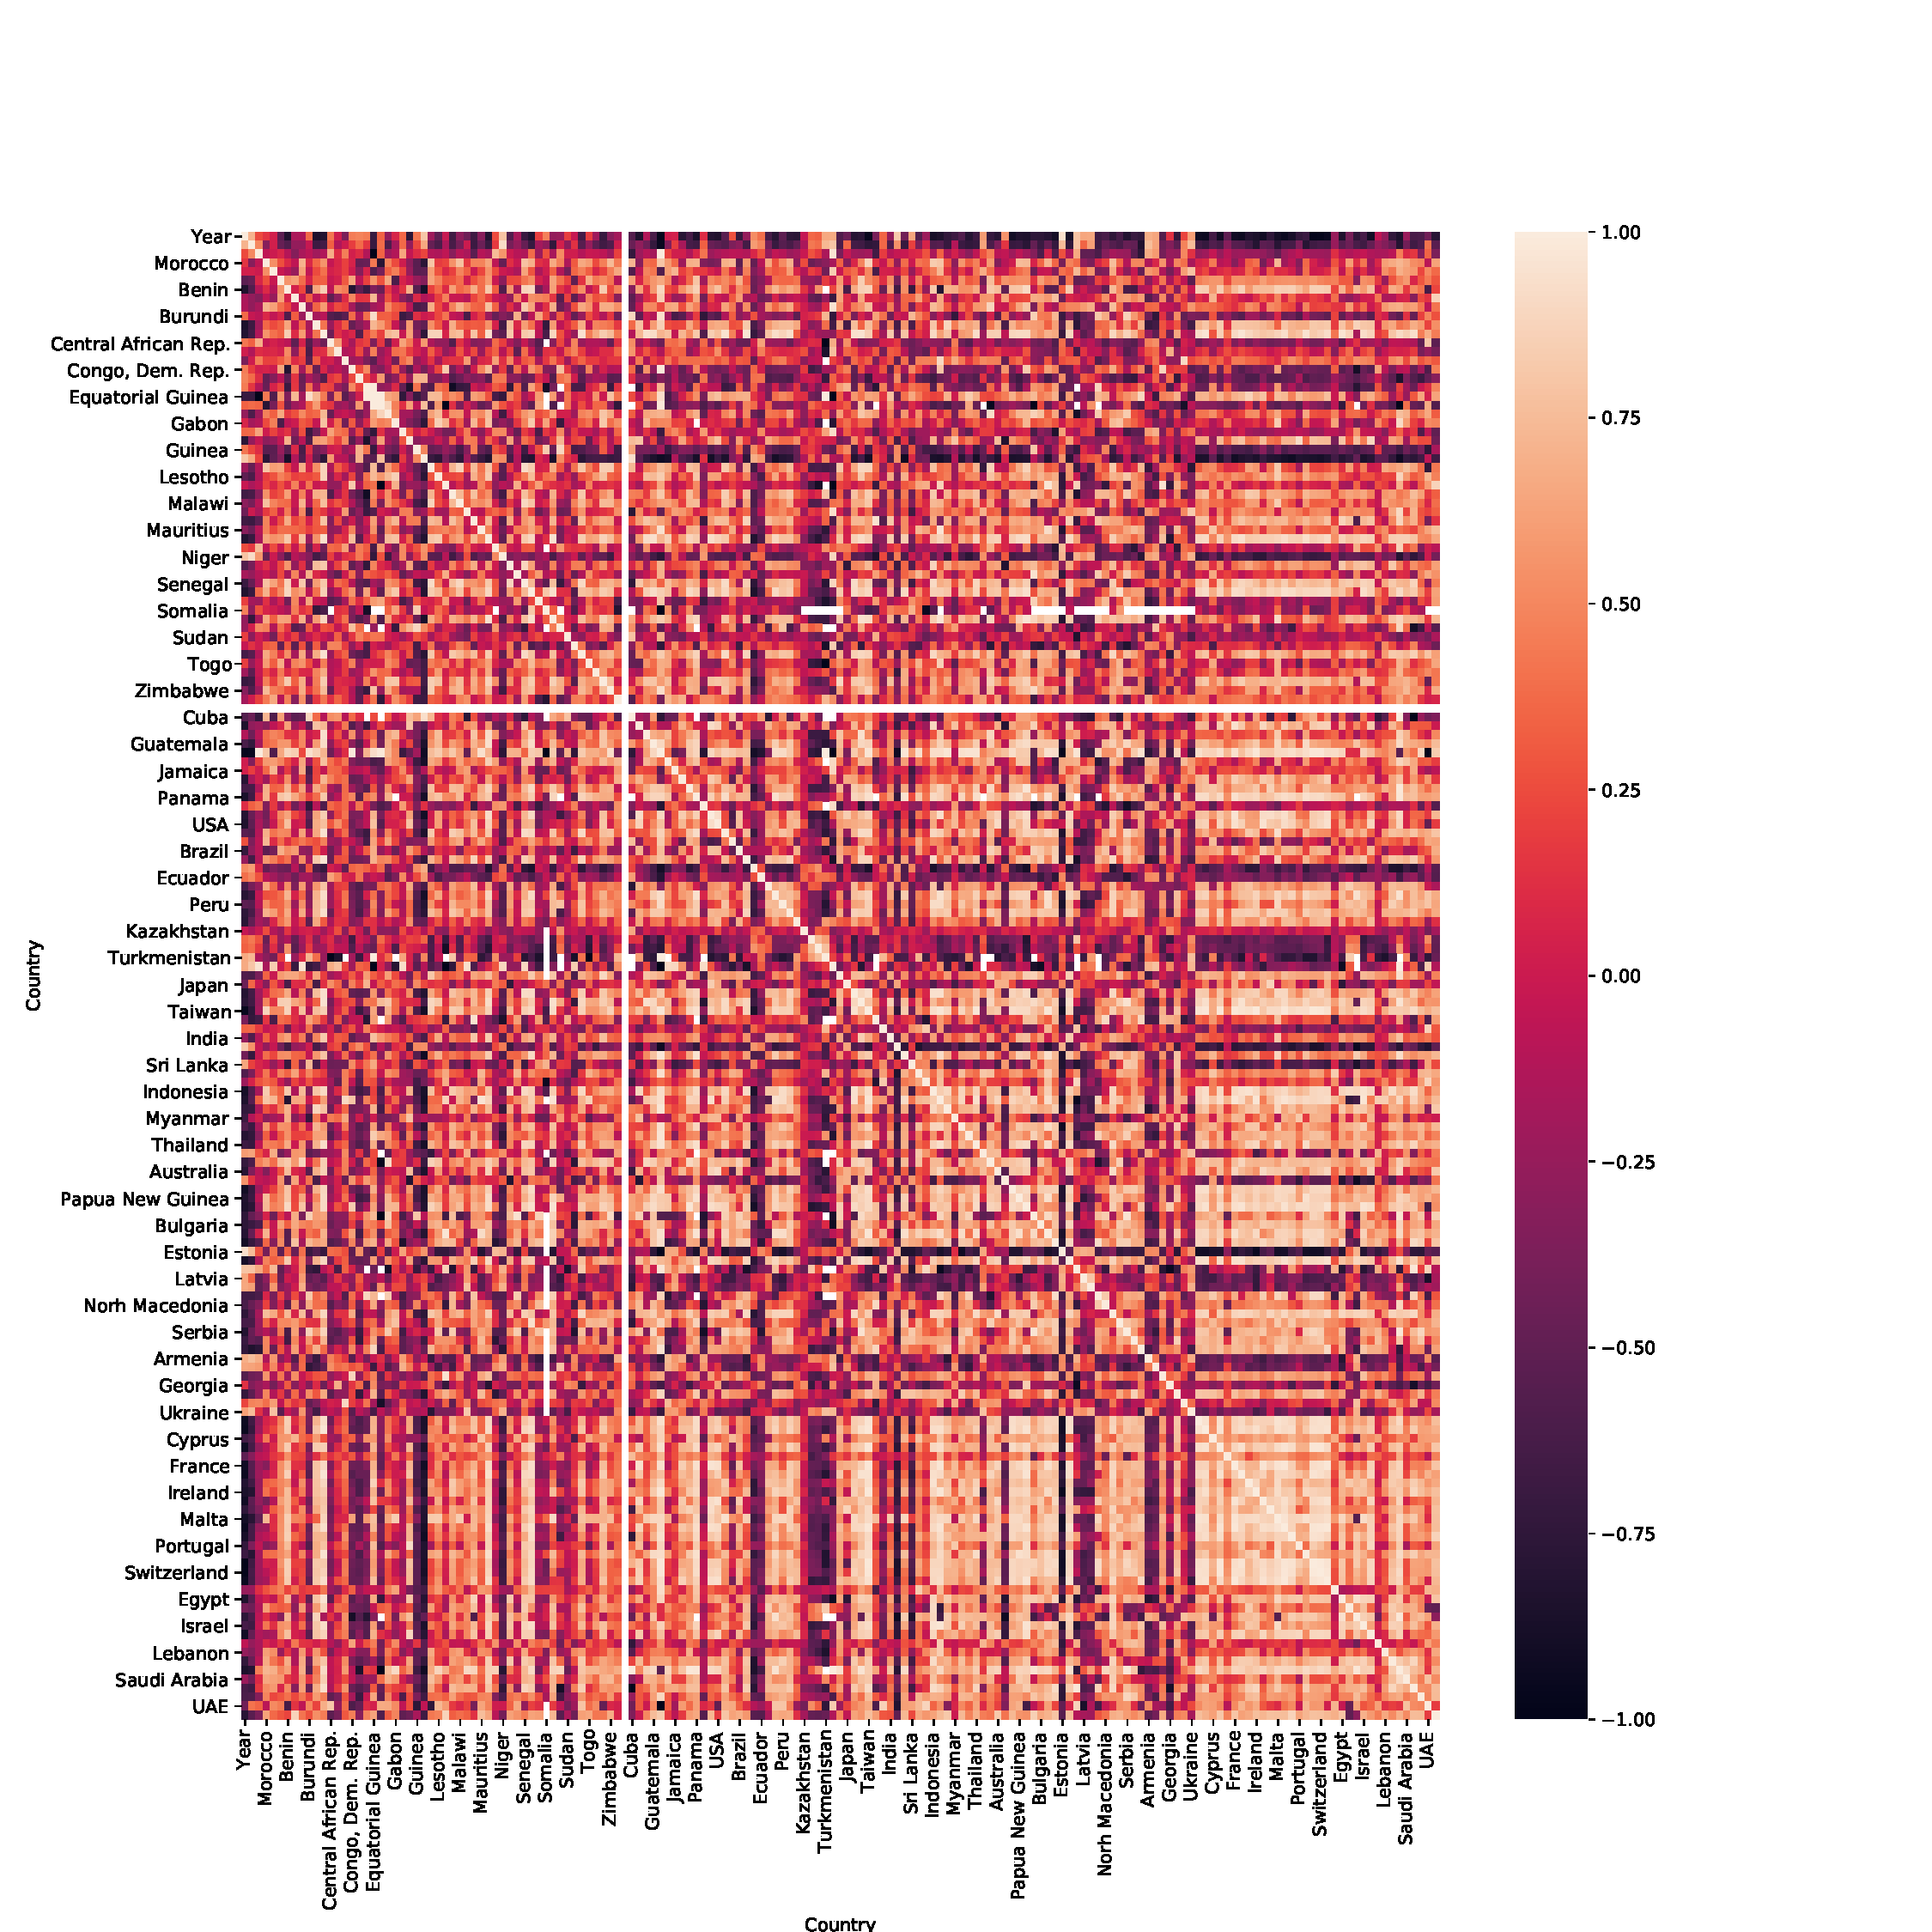
\includegraphics[width=\linewidth,keepaspectratio=true]{../Output/Figures/Milex_Correlations.pdf}
	\end{figure}

    \section*{The Missing Values Problem}

    In order to use PCA and the LASSO, we need to figure out a way to handle missing values in the panel. Here I interpolate values between data points where we have spending information for a country, and also restrict the sample to observations after 1995.

	Beyond this (graph not shown) I then delete any countries which still have a missing value for any year. A lot more could probably done to optimize the size of the balanced panel; we could try to maximize the rectangular filled area in the charts.

	\begin{figure}[h!]
		\centering
		\caption{Missing Values Before Interpolation}
		\label{SIPRI_Missing_Values}	
		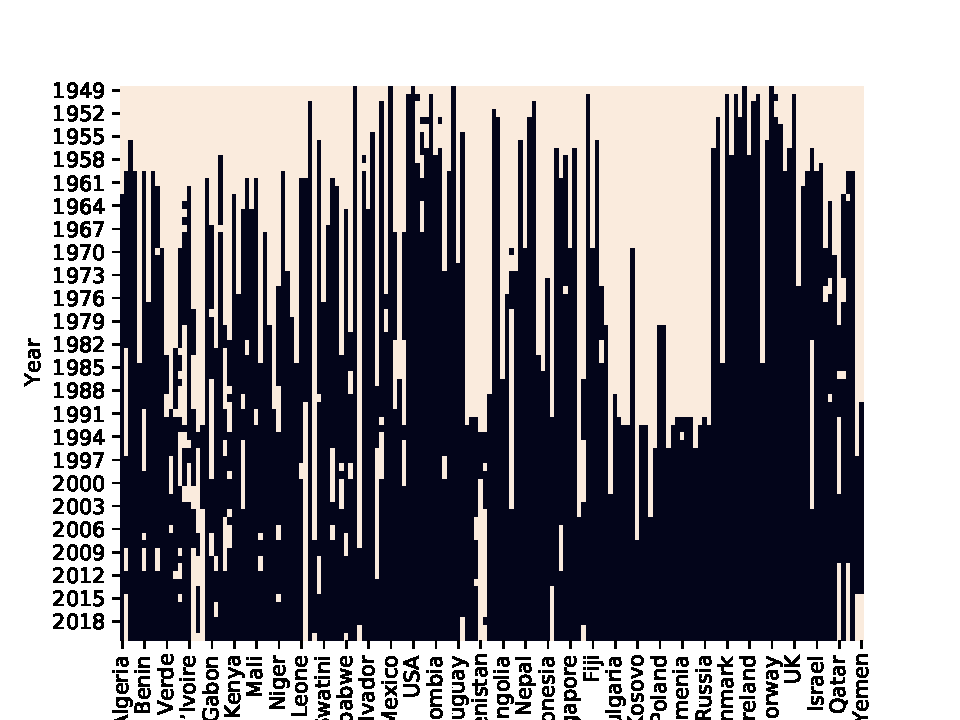
\includegraphics[width=\linewidth,keepaspectratio=true]{../Output/Figures/SIPRI_Missing_Values.pdf}
	\end{figure}

	\begin{figure}[h!]
		\centering
		\caption{Missing Values After Interpolation and Sample Restriction}
		\label{SIPRI_Missing_Values_Inter_Post_1995}	
		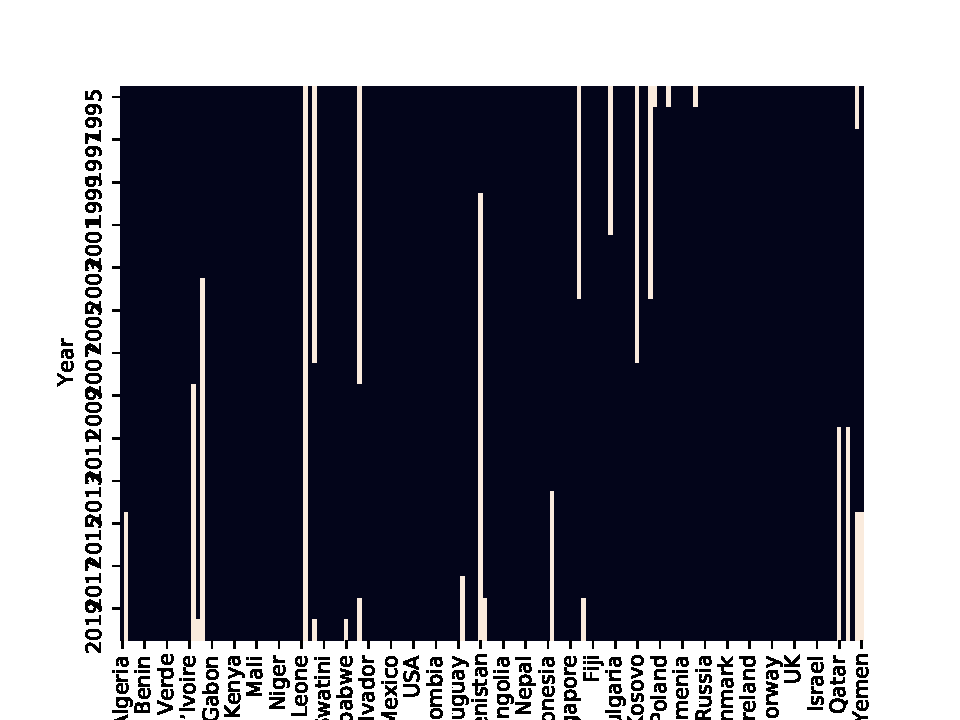
\includegraphics[width=\linewidth,keepaspectratio=true]{../Output/Figures/SIPRI_Missing_Values_Interpolate_Post_1995.pdf}
	\end{figure}

    \newpage \clearpage

    \section*{PCA Results}

    I performed a PCA to see if there were components which explained a large amount of the variation in spending across countries and over time.

	\begin{figure}[h!]
		\centering
		\caption{Military Spending PCA Loadings}
		\label{Milex_Loadings}	
		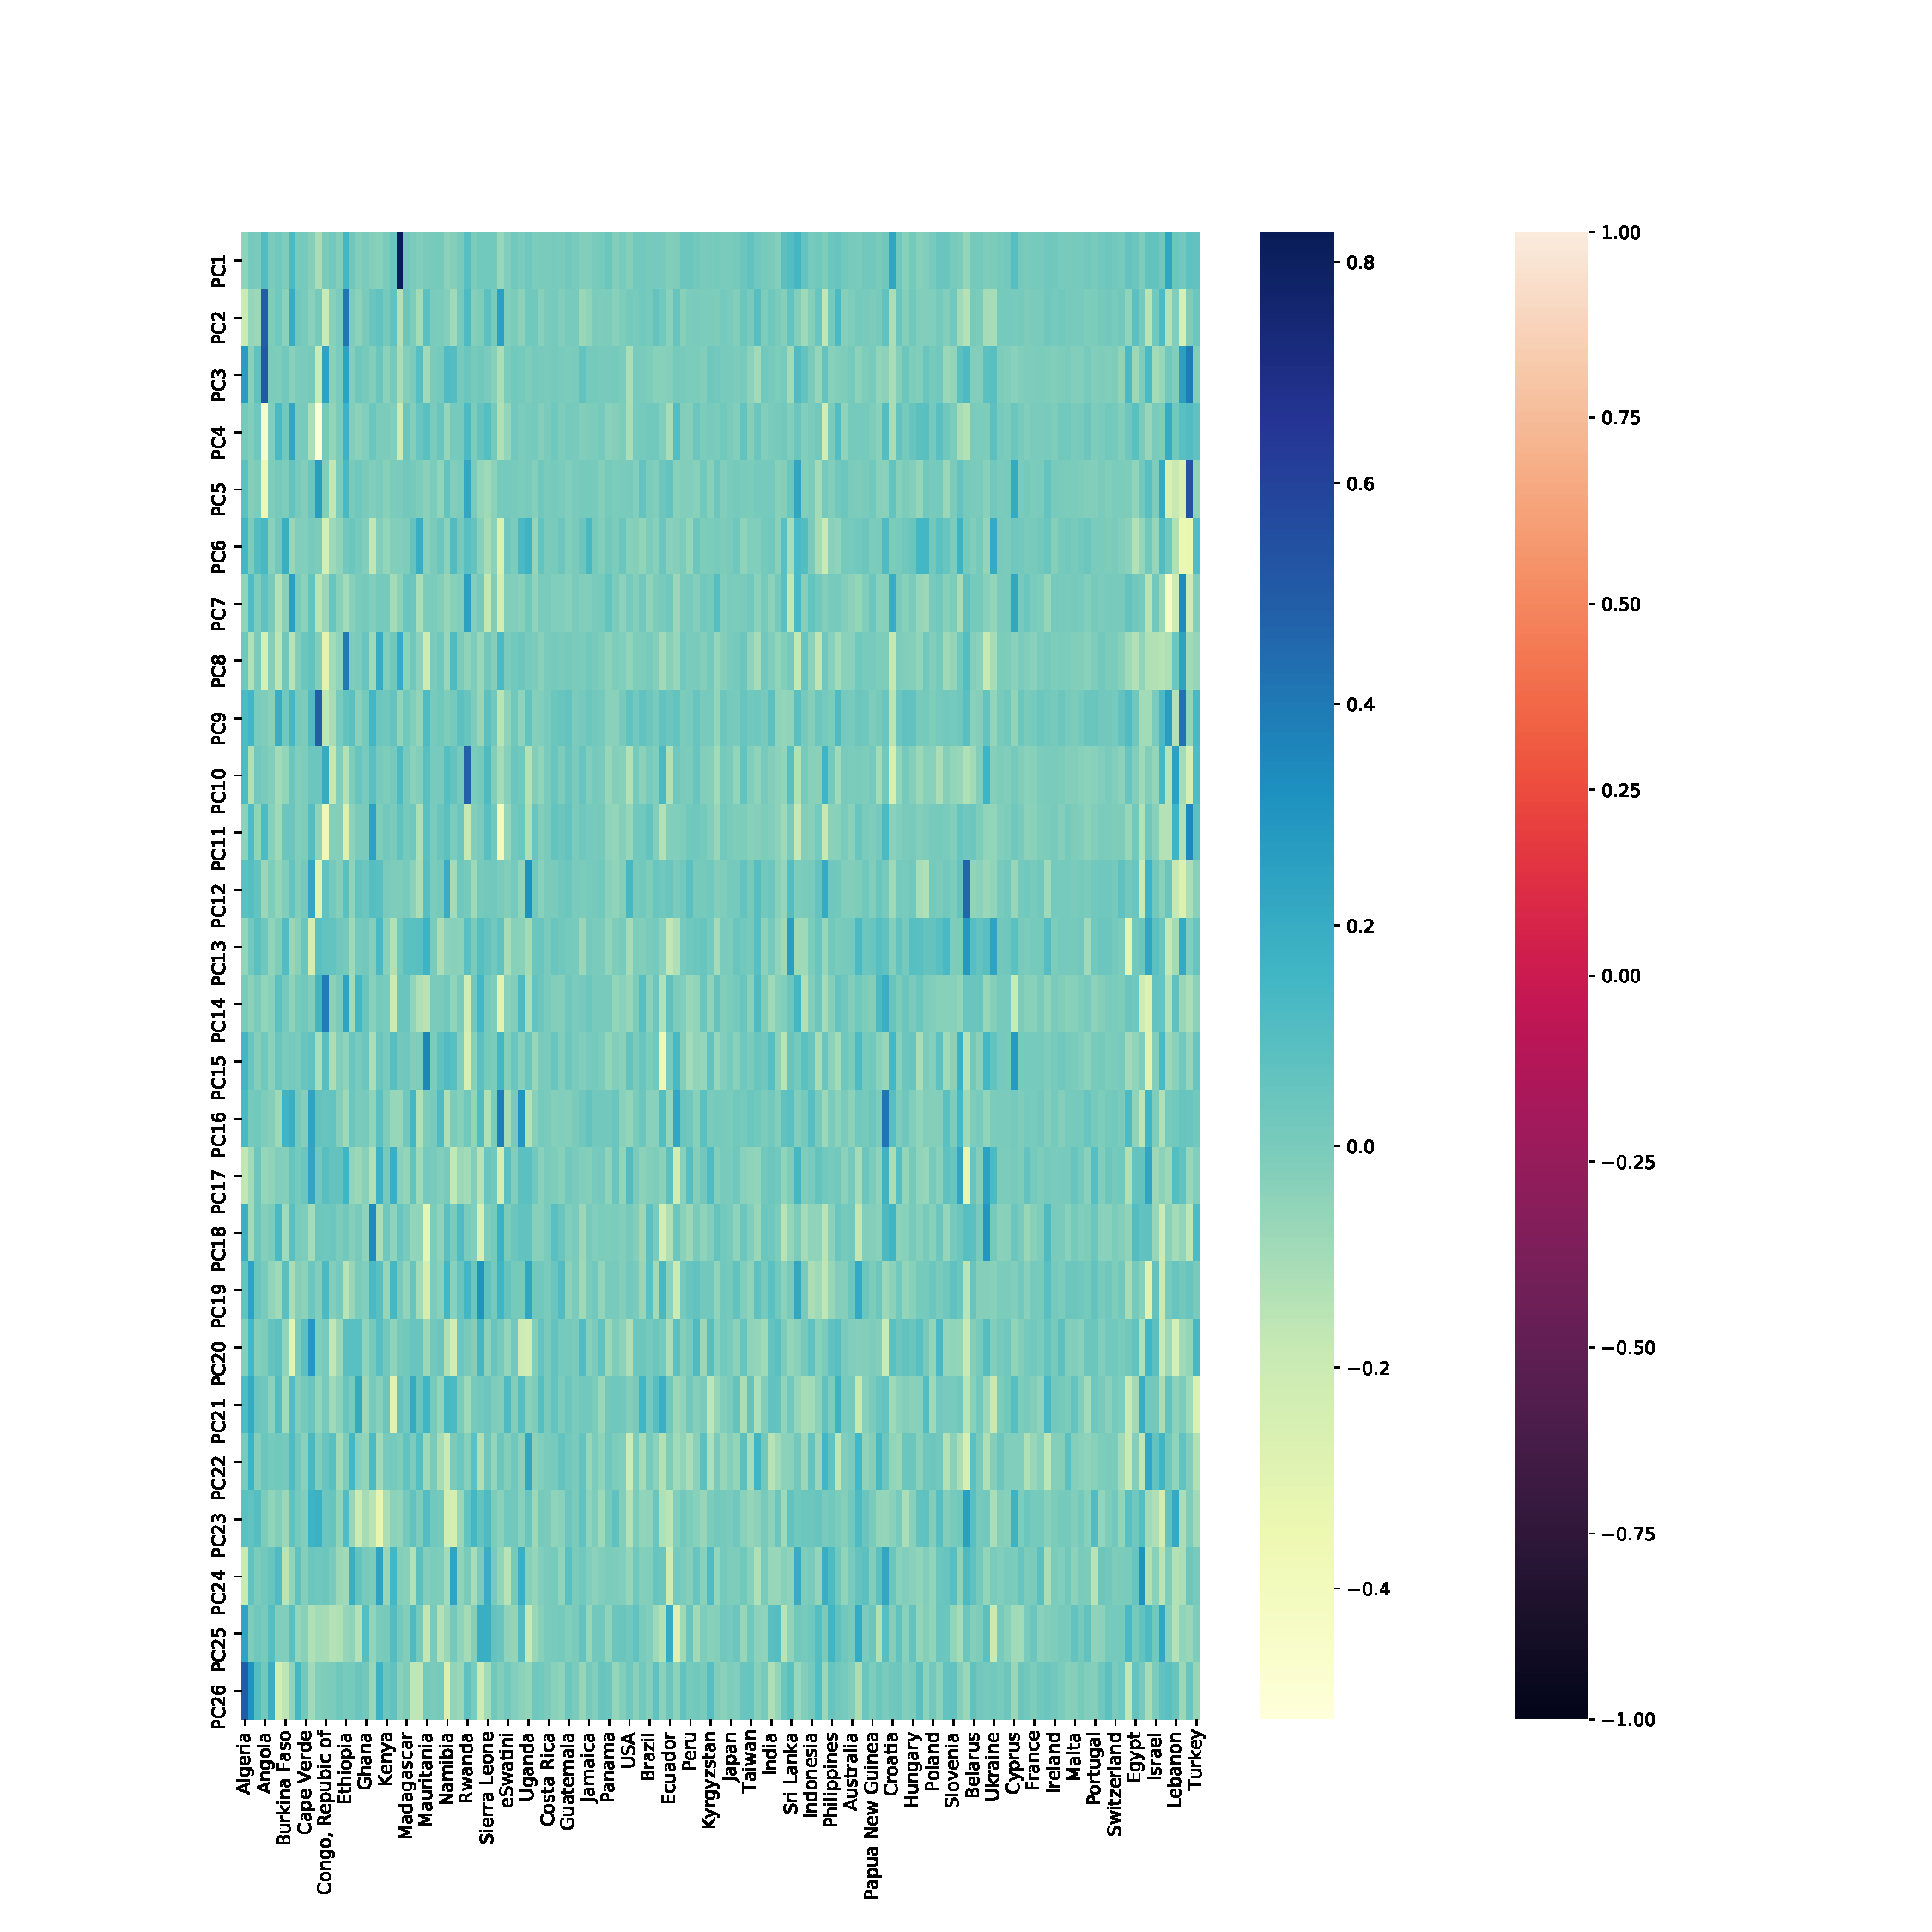
\includegraphics[width=\linewidth,keepaspectratio=true]{../Output/Figures/Milex_Loadings.pdf}
	\end{figure}

    The data is very well summarized with very few principal components.

	\begin{figure}[h!]
		\centering
		\caption{Military Spending PCA Share of Variance Explained}
		\label{Milex_PC_Share_Explained}	
		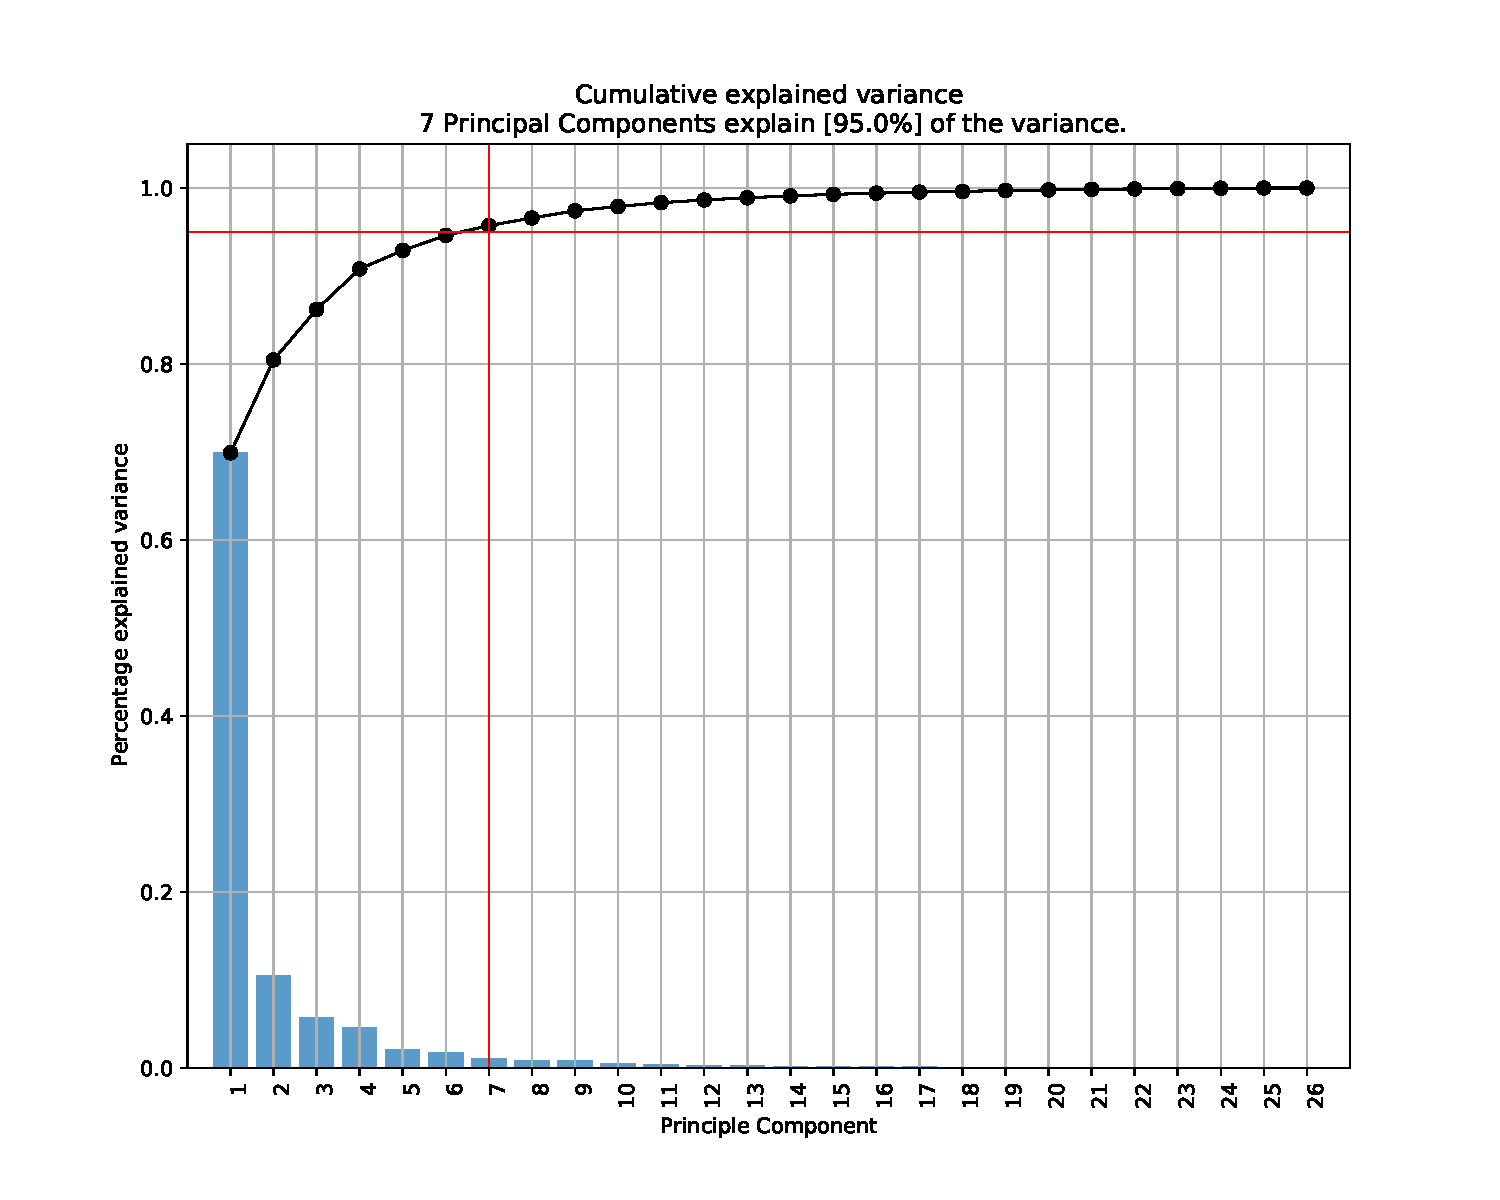
\includegraphics[width=\linewidth,keepaspectratio=true]{../Output/Figures/Milex_PC_Share_Explained.pdf}
	\end{figure}

	\newpage \clearpage

	\section*{LASSO Results}

	Doing the LASSO feels a bit strange, given that we don't really have a "different" dependent variable; we are merely regressing a countries spending on that of other countries. This means that we must impose a bunch of potentially dicey sample restrictions. 
	
	At the moment, I am running a LASSO regression for each individual country across time (so there is a single observation for each time period). The dependent variable is that country's spending per GDP and the independent variables (which may have penalized coefficients) are spending for all the other countries.

	Here are the average coefficients across country regressions.

	% latex table generated in R 4.0.2 by xtable 1.8-4 package
% Thu May 06 13:37:03 2021
\begin{longtable}{rlr}
  \hline
 & Coeff & mean\_coeff \\ 
  \hline
1 & (Intercept) & 0.00 \\ 
  2 & Afghanistan & 0.01 \\ 
  3 & Albania & 0.01 \\ 
  4 & Algeria & 0.00 \\ 
  5 & Angola & 0.00 \\ 
  6 & Argentina & 0.03 \\ 
  7 & Armenia & 0.00 \\ 
  8 & Australia & 0.08 \\ 
  9 & Austria & 0.02 \\ 
  10 & Azerbaijan & 0.00 \\ 
  11 & Bahrain & 0.00 \\ 
  12 & Bangladesh & 0.01 \\ 
  13 & Belarus & 0.00 \\ 
  14 & Belgium & 0.01 \\ 
  15 & Belize & 0.02 \\ 
  16 & Benin & 0.01 \\ 
  17 & Bolivia & 0.05 \\ 
  18 & Botswana & 0.01 \\ 
  19 & Brazil & 0.03 \\ 
  20 & Brunei & 0.00 \\ 
  21 & Bulgaria & 0.00 \\ 
  22 & Burkina Faso & 0.00 \\ 
  23 & Burundi & 0.00 \\ 
  24 & Cambodia & 0.00 \\ 
  25 & Cameroon & 0.03 \\ 
  26 & Canada & 0.02 \\ 
  27 & Cape Verde & 0.05 \\ 
  28 & Central African Rep. & 0.00 \\ 
  29 & Chad & -0.00 \\ 
  30 & Chile & 0.00 \\ 
  31 & China & 0.00 \\ 
  32 & Colombia & 0.00 \\ 
  33 & Congo, Dem. Rep. & 0.00 \\ 
  34 & Congo, Repubic of & 0.01 \\ 
  35 & Costa Rica & 0.00 \\ 
  36 & C�te d�Ivoire & -0.00 \\ 
  37 & Croatia & 0.00 \\ 
  38 & Cyprus & 0.00 \\ 
  39 & Czechia & 0.00 \\ 
  40 & Denmark & 0.01 \\ 
  41 & Dominican Rep. & -0.01 \\ 
  42 & Ecuador & 0.01 \\ 
  43 & Egypt & 0.00 \\ 
  44 & El Salvador & 0.00 \\ 
  45 & Estonia & -0.02 \\ 
  46 & eSwatini & -0.00 \\ 
  47 & Ethiopia & 0.00 \\ 
  48 & Fiji & 0.02 \\ 
  49 & Finland & 0.01 \\ 
  50 & France & 0.01 \\ 
  51 & Gabon & 0.01 \\ 
  52 & Gambia & 0.01 \\ 
  53 & Germany & 0.02 \\ 
  54 & Ghana & 0.01 \\ 
  55 & Greece & 0.01 \\ 
  56 & Guatemala & 0.00 \\ 
  57 & Guinea & -0.00 \\ 
  58 & Guinea-Bissau & 0.00 \\ 
  59 & Guyana & 0.01 \\ 
  60 & Haiti & 0.04 \\ 
  61 & Honduras & 0.00 \\ 
  62 & Hungary & 0.01 \\ 
  63 & India & 0.02 \\ 
  64 & Indonesia & 0.01 \\ 
  65 & Iran & 0.00 \\ 
  66 & Iraq & 0.01 \\ 
  67 & Ireland & 0.01 \\ 
  68 & Israel & 0.00 \\ 
  69 & Italy & 0.00 \\ 
  70 & Jamaica & -0.00 \\ 
  71 & Japan & 0.26 \\ 
  72 & Jordan & -0.01 \\ 
  73 & Kazakhstan & 0.02 \\ 
  74 & Kenya & -0.02 \\ 
  75 & Korea, South & -0.01 \\ 
  76 & Kuwait & 0.00 \\ 
  77 & Kyrgyzstan & 0.01 \\ 
  78 & Latvia & -0.00 \\ 
  79 & Lebanon & 0.00 \\ 
  80 & Lesotho & -0.00 \\ 
  81 & Liberia & 0.00 \\ 
  82 & Lithuania & 0.00 \\ 
  83 & Luxembourg & -0.04 \\ 
  84 & Madagascar & 0.01 \\ 
  85 & Malawi & -0.01 \\ 
  86 & Malaysia & 0.00 \\ 
  87 & Mali & 0.01 \\ 
  88 & Malta & -0.01 \\ 
  89 & Mauritania & -0.00 \\ 
  90 & Mauritius & 0.20 \\ 
  91 & Mexico & 0.09 \\ 
  92 & Moldova & 0.02 \\ 
  93 & Mongolia & 0.01 \\ 
  94 & Morocco & -0.01 \\ 
  95 & Mozambique & -0.00 \\ 
  96 & Myanmar & 0.00 \\ 
  97 & Namibia & -0.00 \\ 
  98 & Nepal & -0.03 \\ 
  99 & Netherlands & 0.01 \\ 
  100 & New Zealand & 0.01 \\ 
  101 & Nicaragua & 0.00 \\ 
  102 & Niger & -0.00 \\ 
  103 & Nigeria & 0.01 \\ 
  104 & Norway & 0.03 \\ 
  105 & Oman & 0.00 \\ 
  106 & Pakistan & 0.01 \\ 
  107 & Panama & 0.02 \\ 
  108 & Papua New Guinea & 0.01 \\ 
  109 & Paraguay & 0.04 \\ 
  110 & Peru & 0.01 \\ 
  111 & Philippines & 0.01 \\ 
  112 & Poland & 0.04 \\ 
  113 & Portugal & 0.00 \\ 
  114 & Romania & 0.00 \\ 
  115 & Russia & 0.01 \\ 
  116 & Rwanda & 0.00 \\ 
  117 & Saudi Arabia & 0.00 \\ 
  118 & Senegal & 0.00 \\ 
  119 & Seychelles & -0.01 \\ 
  120 & Sierra Leone & 0.01 \\ 
  121 & Singapore & 0.01 \\ 
  122 & Slovakia & -0.01 \\ 
  123 & Slovenia & 0.00 \\ 
  124 & South Africa & 0.03 \\ 
  125 & Spain & 0.00 \\ 
  126 & Sri Lanka & 0.00 \\ 
  127 & Sudan & -0.00 \\ 
  128 & Sweden & 0.00 \\ 
  129 & Switzerland & 0.00 \\ 
  130 & Taiwan & 0.01 \\ 
  131 & Tajikistan & 0.00 \\ 
  132 & Tanzania & 0.03 \\ 
  133 & Thailand & 0.03 \\ 
  134 & Togo & 0.01 \\ 
  135 & Trinidad \& Tobago & 0.01 \\ 
  136 & Tunisia & 0.01 \\ 
  137 & Turkey & 0.00 \\ 
  138 & Uganda & 0.00 \\ 
  139 & UK & -0.00 \\ 
  140 & Ukraine & 0.00 \\ 
  141 & Uruguay & 0.01 \\ 
  142 & USA & 0.00 \\ 
  143 & Zambia & 0.01 \\ 
  144 &  &  \\ 
   \hline
\hline
\end{longtable}


	I am not terribly confident that these results are not just pure noise, because I do not see any clear patterns. The sample size restriction to about 25 observations seems too harsh, but necessary in order to include a large amount of other country independent variables in every regression.

	\newpage \clearpage

    \section*{Extension: Textual Analysis}

	If time allows, we could also look into a quick textual analysis of UN resolutions or NATO statements to validate any findings about the importance of ideological or geographic factors.

\end{document}